\documentclass[11pt,a4paper]{article}
\usepackage{fontspec}
\setmainfont{Times New Roman}
\setsansfont{Segoe UI}
\setmonofont{Consolas}
\usepackage[top=0.40in, bottom=0.40in, left=0.68in, right=0.68in, headheight=0pt, headsep=0pt]{geometry}
\usepackage{amsmath,amssymb}
\usepackage{graphicx}
\usepackage{xcolor}
\usepackage{tikz}
\usetikzlibrary{arrows.meta,positioning,calc,decorations.pathreplacing}
\usepackage{tcolorbox}
\usepackage{hyperref}
\usepackage{booktabs}
\usepackage{url}
\usepackage{caption}

\captionsetup[table]{name=Bảng}
\captionsetup[figure]{name=Hình}

\hypersetup{
    colorlinks=true,
    linkcolor=blue!70!black,
    citecolor=blue!70!black,
    urlcolor=blue!70!black
}

% Hộp chú giải sư phạm theo house style
\newtcolorbox{learningobj}{
    colback=blue!3!white,
    colframe=blue!60!black,
    fonttitle=\bfseries\sffamily,
    fontupper=\small,
    title={$\blacktriangleright$ MỤC TIÊU HỌC TẬP},
    arc=1.5mm,
    boxrule=0.8pt,
    left=3mm, right=3mm, top=1.2mm, bottom=1.2mm,
    before skip=1mm, after skip=1.5mm
}

\newtcolorbox{groundbreaking}{
    colback=teal!4!white,
    colframe=teal!60!black,
    fonttitle=\bfseries\sffamily,
    title={$\bigstar$ PHÁT HIỆN THEN CHỐT},
    arc=1.5mm,
    boxrule=0.8pt,
    left=3.5mm, right=3.5mm, top=1.5mm, bottom=1.5mm,
    before skip=1.2mm, after skip=1.5mm
}

\newtcolorbox{physicalinsight}{
    colback=yellow!6!white,
    colframe=orange!75!black,
    fonttitle=\bfseries\sffamily,
    title={$\blacktriangleright$ NHÌN THẤY VẬT LÝ},
    arc=1.5mm,
    boxrule=0.8pt,
    left=3.5mm, right=3.5mm, top=1.5mm, bottom=1.5mm,
    before skip=1.2mm, after skip=1.5mm
}

\renewcommand{\thefigure}{1.4\alph{figure}}

\begin{document}

% ============================================================================
% TRANG 1: MỤC TIÊU HỌC TẬP & CẢNH 1 (RANH GIỚI THỜI GIAN VÀ BƯỚC NHẢY)
% ============================================================================

\section*{1.4 Ý Nghĩa Phần Cứng và Giới Hạn Thời Gian Thực}

Mục 1.3 đã khảo sát chi phí tính toán lý thuyết của từng toán tử biến đổi phổ trên một khung dữ liệu độc lập. Khi chuyển các toán tử đó sang môi trường phần cứng biên xử lý tín hiệu theo dòng liên tục, những câu hỏi cốt lõi về thời gian thực, dung lượng lưu trữ nội vi và mô hình hàng đợi bắt đầu xuất hiện.

\begin{learningobj}
\begin{enumerate}
    \item Các toán tử biến đổi phổ trong Mục 1.3 có chi phí tính toán cho mỗi khung rời rạc, nhưng khi nào kết quả đầu tiên của chuỗi xử lý âm thanh có thể xuất hiện trên mạch vật lý?
    \item 400 mẫu tín hiệu của một khung cửa sổ được lưu trữ ở đâu trong tài nguyên FPGA và chiếm bao nhiêu dung lượng của một khối Block RAM đơn lẻ?
    \item Ma trận ngân hàng bộ lọc Mel kích thước $80 \times 257$ thực tế tiêu tốn bao nhiêu dung lượng lưu trữ trọng số và bao nhiêu phép tính số học mỗi khung?
    \item Việc di chuyển tiền xử lý âm thanh lên phần cứng chuyên dụng có phải là một thắng lợi về thông lượng tính toán so với Edge GPU hay không?
    \item Nếu khối lượng tính toán số học rất nhỏ, điều gì vẫn có thể làm trễ hạn chót 10 ms của bước nhảy khung âm thanh?
    \item Hiện tượng gì xảy ra ở ranh giới 1 giây âm thanh đối với các mẫu dữ liệu cuối cùng, và việc gom cụm khung (batching) tạo ra chi phí trễ thời gian như thế nào?
\end{enumerate}
\end{learningobj}

\subsection*{1. Ranh Giới Thời Gian Khung Đầu Tiên và Nhịp Bước Nhảy}

\textbf{Câu hỏi giai đoạn trước không thể trả lời:} Các toán tử trong Mục 1.3 có chi phí tính toán xác định cho mỗi khung âm thanh rời rạc, nhưng khi nào kết quả đầu tiên thực sự có thể tồn tại trên mạch vật lý?

\begin{figure}[h]
\centering
% fig_1_4a_vi.tex: Trục thời gian tiến trình khung âm thanh (tính theo mili-giây)
\begin{tikzpicture}[
  >=Stealth,
  font=\small,
  timeline/.style={->, thick, black!70},
  tick/.style={black!70, thin},
  framebar/.style={draw=blue!75!black, fill=blue!12, rounded corners=2pt, semithick},
  sharedbar/.style={draw=blue!70!black, fill=blue!20, semithick},
  hopbar/.style={draw=teal!75!black, fill=teal!25, semithick},
  f2bar/.style={draw=blue!50!purple!75!black, fill=blue!50!purple!15, rounded corners=2pt, semithick},
  brace/.style={decorate, decoration={brace, amplitude=4pt, mirror}, thick, black!75}
]

% Tỉ lệ: 1 ms = 0.24 cm. Trục từ 0 đến 50 ms
\def\xscale{0.24}

% Trục thời gian
\draw[timeline] (-0.2, -0.1) -- (51*\xscale, -0.1) node[right, font=\footnotesize] {Thời gian (ms)};

\foreach \t in {0, 10, 20, 25, 30, 35, 40, 45, 50} {
  \draw[tick] (\t*\xscale, -0.05) -- (\t*\xscale, -0.15) node[below, font=\scriptsize] {\t};
}

% Khung 0: 0 đến 25 ms
\draw[framebar] (0*\xscale, 2.3) rectangle (25*\xscale, 2.9);
\node[font=\footnotesize\bfseries, text=blue!85!black] at (12.5*\xscale, 2.6) {Khung 0: Chiều dài 25 ms ($L = 400$ mẫu)};
\node[anchor=west, font=\scriptsize\itshape, text=black!70] at (25.5*\xscale, 2.6) {Mẫu thứ 400 chưa đến trước thời điểm 25 ms};

% Khung 1: 10 đến 35 ms (hai sắc độ: phần dùng chung và bước nhảy mới)
\draw[sharedbar] (10*\xscale, 1.25) rectangle (25*\xscale, 1.85);
\node[font=\scriptsize, text=blue!90!black] at (17.5*\xscale, 1.55) {Dùng chung 240 mẫu};

\draw[hopbar] (25*\xscale, 1.25) rectangle (35*\xscale, 1.85);
\node[font=\scriptsize\bfseries, text=teal!90!black] at (30*\xscale, 1.55) {Bước nhảy: 10 ms};

\node[anchor=west, font=\scriptsize, text=black!75] at (35.5*\xscale, 1.55) {Chiều dài khung: 25 ms (160 mẫu mới)};

% Khung 2: 20 đến 45 ms
\draw[f2bar] (20*\xscale, 0.2) rectangle (45*\xscale, 0.8);
\node[font=\footnotesize, text=black!85] at (32.5*\xscale, 0.5) {20 ms đến 45 ms và $L = 400$};

% Móc ngoặc nhịp khung: dưới đoạn 25 - 35 ms
\draw[brace] (25*\xscale, -0.65) -- (35*\xscale, -0.65);
\node[below=5pt, font=\scriptsize\bfseries, text=black!85] at (30*\xscale, -0.65) {Nhịp khung: 10 ms};

\end{tikzpicture}

\caption{\textbf{Bản chất:} Tiến trình thời gian của các khung âm thanh nối tiếp và cơ chế gối đầu tại tần số lấy mẫu $f_s = 16.000\text{ Hz}$. \textbf{Điểm cần quan sát:} Khung 0 đòi hỏi đúng 25 ms để thu thập đủ 400 mẫu; Khung 1 tái sử dụng 240 mẫu cũ và nhận thêm 160 mẫu mới sau bước nhảy 10 ms; Khung 2 hoàn tất tại 45 ms; nhịp xuất khung sau đó đều đặn rơi vào mỗi chu kỳ 10 ms. \textbf{Ý nghĩa:} Ranh giới vật lý 25 ms là sàn trễ tự nhiên không thể rút ngắn bằng việc tăng tần số xung nhịp; sau khung đầu tiên, toàn bộ chuỗi toán tử phải hoàn tất trong khoảng thời gian khắt khe 10 ms.}
\label{fig:1_4a_timeline}
\end{figure}

Với tần số lấy mẫu $f_s = 16.000\text{ Hz}$ và chiều dài khung $L = 400$ mẫu, thời gian cần thiết để thu thập đủ một khung dữ liệu hoàn chỉnh là:
\[
\frac{L}{f_s} = \frac{400}{16000} = 0{,}025\text{ s} = 25\text{ ms}
\]
Bước nhảy giữa hai khung liên tiếp là $H = 160$ mẫu, tương ứng với khoảng thời gian bước nhảy:
\[
\frac{H}{f_s} = \frac{160}{16000} = 0{,}010\text{ s} = 10\text{ ms}
\]
Hai khung kế tiếp chia sẻ một lượng mẫu âm thanh gối đầu:
\[
L - H = 400 - 160 = 240\text{ mẫu}
\]
Một xung nhịp xử lý nhanh hơn không thể làm dịch chuyển ranh giới vật lý 25 ms này, bởi mẫu thứ 400 đơn giản là chưa xuất hiện từ bộ chuyển đổi tín hiệu trước thời điểm đó. Sau khi khung đầu tiên hoàn tất, mỗi khung tiếp theo phải được bàn giao sau đúng mỗi chu kỳ 10 ms. Khoảng thời gian 10 ms đó phải chứa trọn vẹn toàn bộ chuỗi xử lý: áp cửa sổ Hamming, biến đổi FFT, tính phổ công suất, tổng năng lượng ngân hàng bộ lọc Mel, nén logarit, và mô hình âm học.

\clearpage

% ============================================================================
% TRANG 2: CẢNH 2 (DUNG LƯỢNG BỘ NHỚ LƯU TRỮ VÀ KHỐI BLOCK RAM)
% ============================================================================

\subsection*{2. Nơi Lưu Trữ 400 Mẫu Âm Thanh: Khối Block RAM Nội Vi}

\textbf{Câu hỏi giai đoạn trước không thể trả lời:} 400 mẫu âm thanh của khung quan sát nằm ở đâu trong kiến trúc phần cứng khi dữ liệu liên tục đổ vào?

Xét đúng một ngăn chứa vật lý trên FPGA: một khối Block RAM (BRAM) chuẩn 36 kbit có dung lượng lưu trữ tính theo byte là:
\[
\frac{36 \times 1024}{8} = 4608\text{ byte}
\]
Bộ đệm vòng (ring buffer) dùng để duy trì cửa sổ trượt 400 mẫu số thực dấu phẩy động 32-bit (FP32) cần:
\[
400 \times 4 = 1600\text{ byte}
\]
Tỉ lệ chiếm dụng của bộ đệm vòng so với sức chứa của đúng một khối BRAM đơn lẻ là:
\[
\frac{1600}{4608} \approx 34{,}7\%
\]

\begin{figure}[h]
\centering
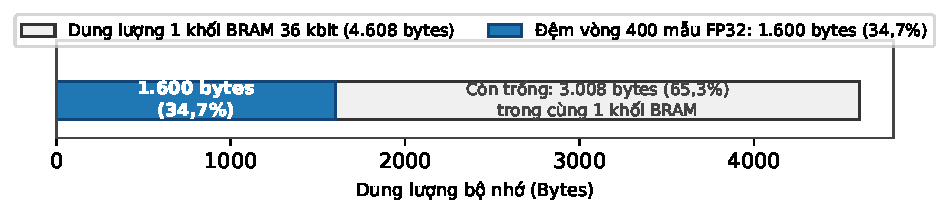
\includegraphics[width=0.86\textwidth]{fig_1_4_bram_vi.pdf}
\caption{\textbf{Bản chất:} Tương quan dung lượng giữa bộ đệm vòng 400 mẫu tín hiệu và sức chứa của một khối Block RAM 36 kbit đơn lẻ. \textbf{Điểm cần quan sát:} Bộ đệm vòng 1.600 byte chiếm 34,7\% dung lượng của khối BRAM 4.608 byte này; phần dung lượng danh định còn lại của khối là 3.008 byte. \textbf{Ý nghĩa:} Bộ đệm vòng 400 mẫu số thực FP32 nằm gọn trong dung lượng danh định 4.608 byte của duy nhất một khối BRAM 36 kbit, với 3.008 byte danh định còn lại của khối đó chưa được phân bổ.}
\label{fig:1_4_bram}
\end{figure}

Tỉ lệ phần trăm 34,7\% này là số byte của bộ đệm chia cho dung lượng danh định in trên tài liệu nhà sản xuất (AMD DS890 v4.10, Bảng 23, thiết bị XCK26). Đây là phép so sánh dung lượng lý thuyết thuần túy, không phải là kết quả đo đếm của một bản thiết kế đã được sắp ráp (placed design) trên chip. Dòng số liệu công bố ``5.1 Mb'' của nhà sản xuất cho 144 khối BRAM trên thiết bị là giá trị làm tròn của phép tính:
\[
144 \times 36\text{ kbit} = 5184\text{ kbit}
\]
Phép nhân số học từ các thông số danh định trên datasheet cho thấy 144 khối BRAM tương ứng với tổng sức chứa lý thuyết:
\[
144 \times 4608\text{ byte} = 663552\text{ byte} = 648\text{ KiB}
\]
Số liệu datasheet ghi nhận 5184 kbit tương đương 648 KiB bộ nhớ BRAM.

\clearpage

% ============================================================================
% TRANG 3: CẢNH 3 (NGÂN HÀNG BỘ LỌC MEL THỰC TẾ LƯU TRỮ VÀ TÍNH TOÁN)
% ============================================================================

\subsection*{3. Ngân Hàng Bộ Lọc Mel Thực Tế: Ma Trận Dày và Cấu Trúc Thưa}

\textbf{Câu hỏi giai đoạn trước không thể trả lời:} Ngân hàng bộ lọc Mel từ Mục 1.3 thực sự lưu trữ bao nhiêu byte và thực hiện bao nhiêu phép tính khi triển khai trên phần cứng?

Nếu triển khai theo kỳ vọng ma trận dày (dense matrix) gồm $80 \times 257$ số thực dấu phẩy động 32-bit, dung lượng lưu trữ bảng trọng số là:
\[
80 \times 257 \times 4 = 82240\text{ byte}
\]
và mỗi khung âm thanh đòi hỏi:
\[
80 \times 257 = 20560\text{ tích mỗi khung}
\]
Tuy nhiên, kiểm tra ma trận do hàm \texttt{create\_mel\_filterbank} xây dựng cho thấy một cấu trúc thưa đặc thù:
\begin{itemize}
    \item \textbf{Hàng chết (toàn số 0):} Có đúng 1 hàng chết (Bộ lọc 2). Kênh này luôn bằng 0, không cần lưu trữ trọng số, không tốn phép nhân và không tốn phép cộng (0 byte, 0 phép nhân, 0 phép cộng).
    \item \textbf{Hàng đơn điểm (one-tap) có trọng số duy nhất bằng 1:} Có 18 hàng thuộc loại này. Năng lượng đầu ra của dải bằng chính công suất phổ tại bin tương ứng ($E_m = P_k$). Phần cứng chỉ cần lưu 1 chỉ số bin dạng số nguyên 32-bit (int32, 4 byte) thay vì lưu trọng số số thực, đồng thời tiêu tốn 0 phép nhân và 0 phép cộng.
    \item \textbf{Hàng đa điểm (multi-bin) có $k$ trọng số dương:} Có 61 hàng thuộc loại này. Mỗi trọng số dương cần lưu 4 byte float32 cho giá trị trọng số cùng 4 byte int32 cho chỉ số bin tương ứng ($k \times 8$ byte). Mỗi hàng này đòi hỏi $k$ phép nhân và $k - 1$ phép cộng.
\end{itemize}

Tổng dung lượng bộ nhớ thực dùng (\texttt{used\_weight\_bytes}) theo mô hình sổ sách của bài học là tổng dung lượng của các phần tử thực tế đó:
\[
0\text{ byte (hàng chết)} + 18 \times 4\text{ byte (hàng đơn điểm)} + 407 \times 8\text{ byte (hàng đa điểm)} = 72 + 3256 = 3328\text{ byte}
\]
So với kỳ vọng ma trận dày 82240 byte, mô hình lưu trữ thực dùng ghi nhận 3328 byte. Cả hai con số đều được tính toán theo quy chuẩn số thực FP32. Tổng khối lượng tính toán thực tế mỗi khung ghi nhận từ lab là \texttt{multiply\_per\_frame} = 407 phép nhân và \texttt{add\_per\_frame} = 346 phép cộng.

\begin{figure}[h]
\centering
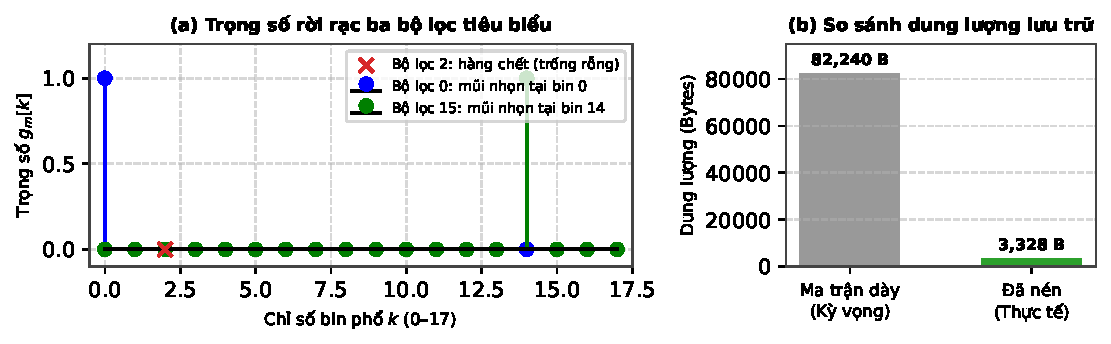
\includegraphics[width=0.86\textwidth]{fig_1_4_bank_vi.pdf}
\caption{\textbf{Bản chất:} Cấu trúc phân bố trọng số của ngân hàng 80 bộ lọc Mel và đối chiếu dung lượng lưu trữ sổ sách. \textbf{Điểm cần quan sát:} Bộ lọc 0 và 15 chỉ gồm một xung đơn vị đơn lẻ; Bộ lọc 2 hoàn toàn rỗng; mô hình lưu trữ thực dùng ghi nhận 3.328 byte so với 82.240 byte của ma trận dày kỳ vọng. \textbf{Ý nghĩa:} Cấu trúc thưa giúp loại bỏ phần lớn gánh nặng tính toán và thu nhỏ bảng tra trọng số, dù 3.328 byte chiếm hơn 72\% dung lượng của một khối BRAM đơn lẻ.}
\label{fig:1_4_bank}
\end{figure}

\begin{physicalinsight}
Bảng trọng số 3.328 byte chiếm tới 72,2\% dung lượng của một khối BRAM 4.608 byte (do đó không thể nhét chung vào phần 3.008 byte còn lại của khối đệm vòng vì $1600 + 3328 = 4928 > 4608$). Tuy nhiên, con số 3.328 byte này rất nhỏ bé khi so với tổng dung lượng 663.552 byte của toàn bộ 144 khối BRAM trên chip. Phép chia dung lượng này là một mô hình tính toán số học trên sổ sách, không phải là một báo cáo tổng hợp mạch vật lý (synthesis report), bởi việc kết nối logic, thanh ghi trung gian và mạch tạo địa chỉ thực tế đòi hỏi các tài nguyên bổ sung trên phần cứng.
\end{physicalinsight}

\clearpage

% ============================================================================
% TRANG 4: CẢNH 4 (ĐỐI CHIẾU THÔNG LƯỢNG VỚI EDGE GPU)
% ============================================================================

\subsection*{4. Đối Chiếu Thông Lượng Tính Toán: Tương Quan Quy Mô}

\textbf{Câu hỏi giai đoạn trước không thể trả lời:} Việc di chuyển khối tiền xử lý âm thanh lên phần cứng chuyên dụng có mang lại thắng lợi về mặt thông lượng tính toán (throughput) hay không?

Với nhịp bước nhảy 10 ms, hệ thống xử lý đúng 100 khung mỗi giây. Thông lượng phép nhân thực tế của ma trận Mel là:
\[
\text{multiply\_per\_second} = 407 \times 100 = 40700\text{ phép nhân/giây}
\]
Các thông số dẫn chiếu từ tài liệu công bố của nhà sản xuất (không phải số đo do lab này tự thực hiện):
\begin{itemize}
    \item NVIDIA Jetson Orin Nano Super công bố định mức cực đại 67 sparse INT8 TOPS tại trần công suất 25 W.
    \item Độ thưa có cấu trúc (structured sparsity 2:4) nhân đôi thông lượng lý thuyết của nhân Tensor Core, do đó giá trị $67 / 2 = 33{,}5\text{ dense INT8 TOPS}$ là một phép tính số học trong cuốn sách này, không phải là một thông số công bố độc lập thứ hai.
\end{itemize}

Đối chiếu quy mô giữa thông lượng tính đổi của GPU và tốc độ nhân ma trận Mel:
\[
\text{quotient\_mac\_as\_one} = \frac{33{,}5 \times 10^{12}}{40700} \approx 823095823{,}10
\]
\[
\text{quotient\_mac\_as\_two} = \frac{33{,}5 \times 10^{12}}{2 \times 40700} \approx 411547911{,}55
\]
Con số 407 trong nhật ký kiểm thử là số phép nhân mỗi khung. 61 hàng đa điểm cần thêm 346 phép cộng, đưa tổng số phép tính của ngân hàng Mel lên 753 thao tác mỗi khung (75.300 thao tác/giây). Thương số thứ nhất so sánh định mức GPU với riêng số phép nhân Mel ($40.700\text{ phép nhân/giây}$). Thương số thứ hai tính theo mẫu số nhân đôi ($2 \times 40.700$). Dù so sánh với riêng phép nhân hay tính cả phép cộng, tỷ lệ quy mô giữa năng lực GPU và tải tính toán Mel đều đứng vững chắc ở bậc hàng trăm triệu lần ($823095823{,}10$ và $411547911{,}55$), và lập luận so sánh hoàn toàn không phụ thuộc vào việc đếm phép tính theo quy ước nào.

\begin{figure}[h]
\centering
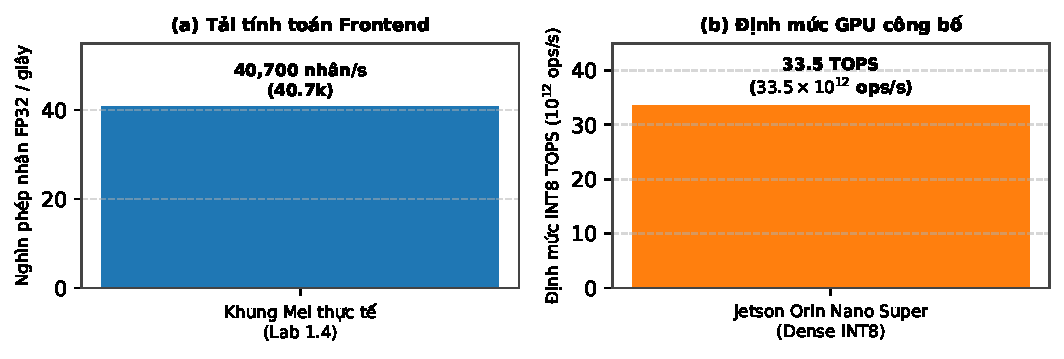
\includegraphics[width=0.86\textwidth]{fig_1_4_rate_vi.pdf}
\caption{\textbf{Bản chất:} Đối chiếu quy mô giữa tốc độ nhân ma trận Mel (FP32) và định mức tính toán công bố của Edge GPU (INT8). \textbf{Điểm cần quan sát:} Khối lượng 40.700 phép nhân/giây chỉ tính riêng cho ma trận Mel; trên trục TOPS của GPU ở panel (b), khối lượng Mel chỉ tương đương $0{,}00000004\text{ TOPS}$, hoàn toàn chìm sát đáy đồ thị so với cột 33,5 dense TOPS; hai thương số quy mô từ nhật ký kiểm thử đều ở bậc hàng trăm triệu lần ($823095823{,}10$ và $411547911{,}55$). \textbf{Ý nghĩa:} Tải tính toán số học của phép nhân Mel hoàn toàn chìm nghỉm trước năng lực tính toán cực đại của GPU, cho thấy phép so sánh thông lượng thuần túy không thể là căn cứ để chuyển đổi sang FPGA.}
\label{fig:1_4_rate}
\end{figure}

Tài liệu AMD DS890 công bố thiết bị XCK26 tích hợp 1248 lát cắt DSP48E2. Tuy nhiên, khối lượng số học tiền xử lý nhỏ bé này không được dùng để suy diễn ra một tỉ lệ phần trăm tải chip hay tần số xung nhịp.

\begin{groundbreaking}
Khối tiền xử lý âm thanh quá nhỏ bé khi đặt cạnh định mức công bố của GPU, do đó một phép so sánh thuần túy về thông lượng tính toán không thể là lý do thuyết phục để biện minh cho việc chuyển đổi kiến trúc sang FPGA.
\end{groundbreaking}

\clearpage

% ============================================================================
% TRANG 5: CẢNH 5 (HÀNG ĐỢI CHIA SẺ VÀ ĐƯỜNG TRUYỀN CHUYÊN DỤNG)
% ============================================================================

\subsection*{5. Cơ Chế Hàng Đợi: Nguyên Nhân Gây Nguy Cơ Trễ Hạn Chót 10 ms}

\textbf{Câu hỏi giai đoạn trước không thể trả lời:} Nếu khối lượng tính toán số học nhỏ đến mức chìm nghỉm như vậy, điều gì vẫn có thể khiến hệ thống vi phạm hạn chót 10 ms của bước nhảy?

Xuất phát từ quan sát về tốc độ tính toán ở Cảnh 4, hai giả thuyết kiến trúc được đặt ra:
\begin{itemize}
    \item \textbf{Giả thuyết A (Đường truyền Edge GPU):} Ngân sách thời gian 10 ms là một hàng đợi tài nguyên chia sẻ chung giữa trình điều khiển micro, hệ điều hành (lập lịch phân phối thời gian CPU/GPU), luồng tiền xử lý frontend, và quá trình suy luận của mô hình âm học. Dù khối lượng số học rất nhỏ, hạn chót 10 ms vẫn có nguy cơ bị vi phạm nếu hàng đợi chia sẻ này phát sinh độ trễ phụ (overhead), nghẽn luồng truyền dữ liệu hoặc bị ngắt quãng bởi các tác vụ hệ thống.
    \item \textbf{Giả thuyết B (Đường truyền FPGA):} Các toán tử tiền xử lý tương tự được bố trí trực tiếp trên các đường dây vật lý độc lập (dedicated wires) tách biệt hoàn toàn khỏi hàng đợi phần mềm. Hạn chót 10 ms chỉ bị vi phạm nếu bản thân chuỗi mắt xích trên các đường dây vật lý đó tốn nhiều hơn 10 ms để hoàn tất.
\end{itemize}

\begin{figure}[h]
\centering
% Figure 1.4b: Phân bổ BRAM trên KV260 và So sánh chồng phần mềm với đường dây chuyên dụng (Bản tiếng Việt)
\begin{tikzpicture}[
  >=Stealth,
  font=\small
]

% ==================== PANEL (a): Phân bổ BRAM trên chip ====================
\begin{scope}[x=1.0cm, y=1.0cm]
  \node (titlea) [font=\bfseries\small, anchor=west] at (0, 4.5) 
    {(a) Phân bổ BRAM trên KV260 ($648\text{ KiB}$ tổng)};

  % Khối bộ đệm vòng âm thanh (trên cùng)
  \node (box1) [
    draw=blue!80!black, fill=blue!12, rounded corners=3pt, thick,
    font=\scriptsize, align=center,
    text width=7.3cm, inner sep=4pt
  ] at (3.8, 3.65) {
    \textbf{\textcolor{blue!90!black}{Bộ đệm vòng âm thanh ($400$ mẫu FP32): $1{.}600\text{ B}$}}\\[0.8mm]
    \scriptsize\textcolor{black!80}{$34{,}7\%$ của 1 khối BRAM ($0{,}2\%$ tổng BRAM trên chip)}
  };

  % Khối ma trận bộ lọc Mel (ở giữa)
  \node (box2) [
    draw=purple!80!black, fill=purple!12, rounded corners=3pt, thick,
    font=\scriptsize, align=center,
    text width=7.3cm, inner sep=4pt,
    below=0.32cm of box1
  ] {
    \textbf{\textcolor{purple!90!black}{Ma trận bộ lọc Mel ($80 \times 257$ FP32): $80{,}3\text{ KiB}$}}\\[0.8mm]
    \scriptsize\textcolor{black!80}{$18$ khối BRAM ($12{,}4\%$ tổng BRAM) $\implies$ $0$ truy xuất DDR}
  };

  % Khối BRAM còn trống cho mô hình nơ-ron (dưới cùng)
  \node (box3) [
    draw=teal!80!black, fill=teal!12, rounded corners=3pt, thick,
    font=\scriptsize, align=center,
    text width=7.3cm, inner sep=4pt,
    below=0.32cm of box2
  ] {
    \textbf{\textcolor{teal!90!black}{Khoảng trống cho mô hình nơ-ron: $566{,}1\text{ KiB}$ ($87{,}4\%$ BRAM)}}\\[0.8mm]
    \scriptsize\textcolor{black!80}{$126$ khối BRAM ($566{,}1\text{ KiB}$) $+$ $64$ khối UltraRAM ($2{,}25\text{ MiB}$)}
  };

  % Chú thích tổng quan dưới panel (a)
  \node (summa) [
    font=\scriptsize, align=center, text=black!75, text width=7.5cm,
    below=0.22cm of box3
  ] {
    Tổng SRAM AMD XCK26: $5{,}1\text{ Mb}$ BRAM $+$ $18{,}0\text{ Mb}$ UltraRAM
  };
\end{scope}

% Đường vách ngăn phân chia
\draw[gray!35, thick, dashed] (8.0, -0.3) -- (8.0, 4.7);

% ==================== PANEL (b): Chồng phần mềm dùng chung vs Đường dây chuyên dụng ====================
\begin{scope}[xshift=8.4cm, x=1.0cm, y=1.0cm]
  \node[font=\bfseries\small, anchor=west] at (0, 4.5) 
    {(b) Nhịp thực thi: Rung pha dùng chung so với Đường dây chuyên dụng};

  % Nhãn đường GPU
  \node[font=\scriptsize\bfseries, text=orange!95!black, anchor=west] at (0.1, 4.0) {
    GPU biên: Chồng phần mềm dùng chung
  };
  % Hộp bao ngoài đường GPU
  \draw[draw=orange!80!black, fill=orange!5, thick, rounded corners=3pt] (0, 2.55) rectangle (8.0, 3.75);
  
  % Chuỗi các bước trong GPU
  \node[draw=orange!70!black, fill=white, rounded corners=2pt, font=\tiny, align=center, text width=1.2cm] at (1.0, 3.15) {Bộ đệm\\DMA micro};
  \draw[->, orange!80!black, semithick] (1.7, 3.15) -- (2.0, 3.15);
  \node[draw=red!70!black, fill=red!8, rounded corners=2pt, font=\tiny, align=center, text width=1.7cm] at (2.95, 3.15) {Ngắt HĐH \&\\hàng đợi driver};
  \draw[->, orange!80!black, semithick] (3.9, 3.15) -- (4.2, 3.15);
  \node[draw=orange!70!black, fill=white, rounded corners=2pt, font=\tiny, align=center, text width=1.4cm] at (5.0, 3.15) {Khởi chạy\\kernel tính toán};
  \draw[->, orange!80!black, semithick] (5.8, 3.15) -- (6.1, 3.15);
  \node[draw=red!80!black, fill=red!15, rounded corners=2pt, font=\tiny\bfseries, align=center, text width=1.5cm] at (7.0, 3.15) {Rung pha trễ\\$\Delta t > 0$};

  % Nhãn đường FPGA
  \node[font=\scriptsize\bfseries, text=teal!95!black, anchor=west] at (0.1, 2.05) {
    FPGA không gian: Đường dây silicon chuyên dụng
  };
  % Hộp bao ngoài đường FPGA
  \draw[draw=teal!80!black, fill=teal!5, thick, rounded corners=3pt] (0, 0.65) rectangle (8.0, 1.85);

  % Chuỗi các bước trong FPGA
  \node[draw=teal!70!black, fill=white, rounded corners=2pt, font=\tiny, align=center, text width=1.2cm] at (1.1, 1.25) {Đường dây\\trực tiếp I2S};
  \draw[->, teal!80!black, semithick] (1.85, 1.25) -- (2.25, 1.25);
  \node[draw=teal!70!black, fill=teal!12, rounded corners=2pt, font=\tiny, align=center, text width=2.4cm] at (3.65, 1.25) {Đường ống DSP chuyên dụng\\$N_{\text{clk}}$ chu kỳ hằng số};
  \draw[->, teal!80!black, semithick] (5.0, 1.25) -- (5.4, 1.25);
  \node[draw=green!80!black, fill=green!15, rounded corners=2pt, font=\tiny\bfseries, align=center, text width=1.9cm] at (6.5, 1.25) {Không rung pha HĐH\\$\Delta t = 0\text{ ns}$ tất định};

  % Chú thích dưới panel (b)
  \node[font=\scriptsize, align=center, text=black!75, text width=8.0cm] at (4.0, 0.05) {
    Đường dây phần cứng độc quyền đáp ứng hạn chót $10\text{ ms}$ trên mọi chu kỳ
  };
\end{scope}

\end{tikzpicture}

\caption{\textbf{Bản chất:} So sánh mô hình hàng đợi chia sẻ tài nguyên (Edge GPU) và mô hình đường truyền dữ liệu chuyên dụng (FPGA). \textbf{Điểm cần quan sát:} Trên Edge GPU, toàn bộ trình điều khiển, hệ điều hành, tiền xử lý và mô hình cùng tranh chấp hạn ngạch thời gian 10 ms; trên FPGA, các toán tử được kết nối bằng đường dây vật lý độc lập. \textbf{Ý nghĩa:} Sự khác biệt kiến trúc nằm ở cơ chế quản lý hàng đợi và tính độc lập của luồng dữ liệu chứ không nằm ở việc rút ngắn thời gian tính toán của từng phép nhân.}
\label{fig:1_4b_queues}
\end{figure}

\begin{physicalinsight}
Khối lượng số học không quyết định việc bảo toàn hạn chót; việc chia sẻ tài nguyên trong hàng đợi có thể gây trễ; chương này chưa có số đo trên mạch để chốt lại kết luận đó.
\end{physicalinsight}

\clearpage

% ============================================================================
% TRANG 6: CẢNH 6 (RANH GIỚI 1 GIÂY, GOM CỤM LÔ VÀ CẦU NỐI MỤC 1.5)
% ============================================================================

\subsection*{6. Ranh Giới Một Giây Âm Thanh và Chi Phí Độ Trễ Gom Cụm}

\textbf{Câu hỏi giai đoạn trước không thể trả lời:} Điều gì còn lại ở ranh giới kết thúc 1 giây âm thanh, và kỹ thuật gom cụm khung (batching) tác động như thế nào đến độ trễ hệ thống?

Xét một đoạn tín hiệu âm thanh có thời lượng chuẩn 1 giây, gồm $16.000$ mẫu tại $f_s = 16.000\text{ Hz}$. Điểm bắt đầu hợp lệ cuối cùng của một khung $L = 400$ mẫu là bội số lớn nhất của bước nhảy $H = 160$ mẫu thỏa mãn điều kiện không vượt quá giới hạn $16000 - 400 = 15600$:
\[
97 \times 160 = 15520
\]
Do đó, các khung hợp lệ chạy từ Khung 0 đến Khung 97, tạo thành tổng cộng \texttt{frames\_in\_one\_second} = 98 khung âm thanh. Khung cuối cùng (Khung 97) bắt đầu tại mẫu 15520 và kết thúc tại:
\[
15520 + 400 = 15920
\]
Phần đuôi dữ liệu còn lại ở cuối giây âm thanh gồm:
\[
16000 - 15920 = 80\text{ mẫu}
\]
Phần 80 mẫu dôi dư này không bao giờ đủ 400 mẫu để cấu thành một khung hợp lệ mới nếu không có các biện pháp chèn số 0 giả định.

\begin{figure}[h]
\centering
% fig_1_4_tail_vi.tex: Khung cuoi trong 1 giay am thanh va phan mau duoi doi du
\begin{tikzpicture}[
  >=Stealth,
  font=\small,
  timeline/.style={->, thick, black!75},
  tick/.style={black!70, thin},
  framebar/.style={draw=blue!75!black, fill=blue!15, rounded corners=2pt, semithick},
  tailbar/.style={draw=orange!85!black, fill=orange!25, rounded corners=2pt, semithick},
  brace/.style={decorate, decoration={brace, amplitude=4pt}, thick, black!75}
]

% Trục thời gian tổng quát cho 1 giây âm thanh (16.000 mẫu = 1000 ms)
\draw[timeline] (0, 0) -- (14.2, 0) node[right, font=\footnotesize] {Mẫu tín hiệu};

% Điểm mốc 0, khung 0
\draw[tick] (0, 0.1) -- (0, -0.1) node[below, font=\scriptsize] {0};
\draw[framebar] (0, 0.4) rectangle (1.2, 1.1);
\node[font=\scriptsize, text=blue!90!black] at (0.6, 0.75) {Khung 0};

% Dấu ngắt quãng (khung 1 đến 96)
\node[font=\normalsize, text=black!50] at (3.5, 0.75) {$\dots\dots$};
\node[font=\scriptsize, text=black!65] at (3.5, 0.25) {98 khung hợp lệ (Khung 0 đến Khung 97)};

% Phóng lớn đoạn cuối từ mẫu 15.000 đến 16.000
\draw[tick] (5.8, 0.1) -- (5.8, -0.1) node[below, font=\scriptsize] {15.000};
\draw[tick] (7.5, 0.1) -- (7.5, -0.1) node[below, font=\scriptsize] {15.520};
\draw[tick] (12.2, 0.1) -- (12.2, -0.1) node[below, font=\scriptsize] {15.920};
\draw[tick] (13.2, 0.1) -- (13.2, -0.1) node[below, font=\scriptsize] {16.000};

% Khung 97: bắt đầu tại mẫu 15520, kết thúc tại mẫu 15920 (chiều dài L = 400 mẫu = 25 ms)
\draw[framebar] (7.5, 0.4) rectangle (12.2, 1.1);
\node[font=\scriptsize\bfseries, text=blue!90!black, align=center] at (9.85, 0.75) {Khung 97: 15.520 đến 15.920\\($L = 400$ mẫu)};

% Phần mẫu dôi dư (đuôi): 15920 đến 16000 (80 mẫu = 5 ms)
\draw[tailbar] (12.2, 0.4) rectangle (13.2, 1.1);

% Chú thích phần mẫu dôi dư
\draw[->, thick, orange!85!black] (12.7, 1.2) -- (12.7, 1.7) node[above, font=\scriptsize\bfseries, text=orange!90!black, align=center] {Đuôi 80 mẫu dôi dư\\(chưa đủ 400 mẫu cho khung mới)};

% Móc ngoặc chú thích thời gian khung 97
\draw[brace] (7.5, 1.2) -- (12.2, 1.2);
\node[above=4pt, font=\scriptsize, text=black!85] at (9.85, 1.2) {25 ms};

% Dòng ghi chú về độ trễ gom lô (batch)
\node[anchor=west, font=\footnotesize, text=black!90] at (0.2, -0.85) {batch = 1 là lựa chọn độ trễ. Gom cụm $B = 8$ khung tích lũy thêm $(8 - 1) \times 10\text{ ms} = 70\text{ ms}$ trước khi khung đầu được xử lý.};

\end{tikzpicture}

\caption{\textbf{Bản chất:} Ranh giới phân khung ở cuối 1 giây âm thanh và phần mẫu dôi dư không đủ điều kiện tạo khung. \textbf{Điểm cần quan sát:} Khung thứ 98 (Khung 97) kết thúc tại mẫu 15.920; 80 mẫu cuối cùng từ 15.920 đến 16.000 bị bỏ sót vì không đủ chiều dài 400 mẫu; việc gom lô $B=8$ phát sinh thêm 70 ms chờ đợi. \textbf{Ý nghĩa:} batch = 1 là lựa chọn đánh đổi độ trễ: gom thêm mỗi khung làm trễ thêm 10 ms; một lô $B = 8$ khung tích lũy thêm 70 ms trước khi khung đầu tiên được đưa vào xử lý.}
\label{fig:1_4_tail}
\end{figure}

Trong kiến trúc xử lý luồng thời gian thực, việc chờ đợi tích lũy $B$ khung để gom thành một lô (batch) sẽ làm gia tăng thêm một khoảng trễ thời gian vật lý:
\[
\Delta t_{\text{batch}} = (B - 1) \times 10\text{ ms}
\]
Cụ thể, một cấu hình gom lô kích thước $B = 8$ khung làm trễ thêm $(8 - 1) \times 10\text{ ms} = 70\text{ ms}$ tích lũy trước khi khung đầu tiên được chuyển đến bộ xử lý. batch = 1 là lựa chọn độ trễ để tránh khoảng thời gian chờ tích lũy hàng đợi này.

\subsection*{Cầu Nối Sang Mục 1.5: Ba Câu Hỏi Mở Về Ranh Giới Phần Cứng}

Phân tích kiến trúc trong mục này để lại ba câu hỏi mở cần giải quyết bằng thực nghiệm đo đạc:
\begin{enumerate}
    \item Điều gì sẽ xảy ra với độ phân giải tần số và dung lượng bộ đệm nếu chiều dài khung cửa sổ bị cắt giảm một nửa ($L = 200$ mẫu thay vì 400 mẫu)?
    \item Điều gì sẽ xảy ra với băng thông dữ liệu và kích thước FFT nếu tín hiệu âm thanh đầu vào được lấy mẫu ở tần số chuẩn $48\text{ kHz}$ thay vì $16\text{ kHz}$?
    \item Điều gì sẽ xảy ra với hiệu năng tính toán và diện tích mạch nếu hệ thống giữ nguyên bảng trọng số ma trận dày $80 \times 257$ thay vì lược bỏ và chỉ lưu các trọng số thực dùng?
\end{enumerate}

Toàn bộ các giá trị tính toán và dữ liệu đo đạc thực nghiệm trong mục này được trích xuất từ nhật ký kiểm thử \texttt{results/lab14/20261005T230515Z/stdout.log} (với mã băm toàn vẹn được lưu giữ trong tập tin kiểm soát \texttt{results/SHA256SUMS}), bảng thông số kỹ thuật kiến trúc AMD/Xilinx DS890 v4.10 (Bảng 23, dòng thiết bị XCK26), và tài liệu định mức công bố của NVIDIA Jetson Orin Nano Super.

\end{document}
